% ICME 2027 submission draft. Compile with the IEEE conference template (IEEEtran.cls, conference option).
% Numbers marked \todo{} are filled from studies/footprint/0{1,2}-*/results after the server runs finish.
\documentclass[conference]{IEEEtran}
\usepackage{amsmath,amssymb,amsthm,booktabs,graphicx,multirow,xcolor}
\usepackage[hidelinks]{hyperref}
\newcommand{\todo}[1]{\textcolor{red}{[#1]}}
\newtheorem{proposition}{Proposition}
\newtheorem{lemma}{Lemma}
\newcommand{\sinc}{\operatorname{sinc}}

\title{Scale as a Footprint: Analytic Cell Responses for Arbitrary-Scale Super-Resolution Beyond the Training Manifold}
\author{\IEEEauthorblockN{Anonymous ICME submission}}

\begin{document}
\maketitle

\begin{abstract}
Arbitrary-scale super-resolution (ASSR) decoders are conditioned on the target pixel size, or \emph{cell}, which they read as a learned input token. We show that this token is only defined on the training manifold. Training always uses equal vertical and horizontal cells, so the per-axis cell response of LIIF- and LTE-style decoders is not identified by the data and is left to initialisation; it becomes arbitrary as soon as the scale is asymmetric, the output is coarser than the input, or the scale leaves the training range. We instead treat the cell as a physical footprint and write its effect in analytically: the output pixel is the exact mean of a local Fourier field over its footprint, which reduces to a separable $\sinc$ attenuation of every basis function. A frequency-resolved analysis explains why this choice is invisible at the symmetric scales that training covers (four decoder designs share one recovery profile there and capacity only improves bands near and above the input Nyquist limit) and why it matters outside them. With a linear readout the footprint integral is exact, so a $2{\times}2$ box average of the $\times 4$ output equals the $\times 2$ output by construction, and asymmetric, downscaled and out-of-range queries need no augmentation. On four benchmarks the footprint decoder matches LTE at symmetric scales, is the only decoder whose true per-axis cell beats a swapped one, and, trained only for upscaling, downscales at 42.8\,dB against the box average where LTE reaches 30.2\,dB and LIIF 23.9\,dB. The same analysis explains LTE's 0.9--3.6\,dB seed-to-seed swings at asymmetric scales and yields a zero-cost repair worth 1.33\,dB. All predictions were registered before the experiments.
\end{abstract}

\begin{IEEEkeywords}
arbitrary-scale super-resolution, implicit neural representation, scale conditioning, anti-aliasing
\end{IEEEkeywords}

\section{Introduction}
Continuous-coordinate decoders~\cite{chen2021liif,lee2022lte} reconstruct an image at any output grid by querying encoder features at continuous positions. Because the same continuous field must serve every output resolution, the decoder is also told the target pixel size: LIIF concatenates the cell to its input~\cite{chen2021liif}, LTE maps it to a phase~\cite{lee2022lte}, and later designs attach it to attention, operators or splats~\cite{cao2023ciaosr,wei2023srno,hu2024gaussiansr}. In all of these the cell is a \emph{token}: a vector whose meaning the network learns from data.

This paper starts from a simple observation about that data. Training samples a scale $s$ and downsamples a square crop by $s$ on both axes, so the decoder only ever sees cells with $c_x=c_y$. For any decoder that reads the cell through a linear layer, the loss is then invariant to moving weight between the two cell inputs (Proposition~\ref{prop:ident}); which response the model gives to $c_x\neq c_y$ is decided by the random initialisation, not by training. The same holds for cells coarser than an input pixel (downscaling) and, in practice, for scales outside the training range, where the official LTE implementation clips the cell~\cite{lee2022lte}. These are not corner cases: anisotropic voxels in medical volumes, display adaptation and resampling pipelines all query a continuous representation off the symmetric training manifold.

We argue that the cell should not be a token but a \emph{footprint}. An output pixel is an integral of the continuous image over its support; for a local Fourier field that integral is closed-form and separable, $\sinc(\omega_x c_x/2)\sinc(\omega_y c_y/2)$ per basis function. Writing it in analytically fixes the per-axis response for every cell, symmetric or not, inside or outside the training range. Our contributions are:
\begin{enumerate}
\item \textbf{Where decoder design cannot matter.} With a frequency axis normalised by the input Nyquist limit, $u=2sr$, four decoder designs share one recovery profile at symmetric in-range scales (spread $\le 0.019$), and capacity improves recovery only from $u\approx0.75$ upward. Reading the cell differently is invisible where training identifies it; this is the first prediction of the footprint view, not a failure of it.
\item \textbf{Identifiability and an exact footprint decoder.} We prove that token-style cell conditioning is not identified under symmetric training, and we give a footprint-exact local Fourier decoder whose linear readout makes the footprint mean exact (Proposition~\ref{prop:exact}), with cross-scale consistency as a corollary.
\item \textbf{Registered experiments beyond the manifold.} Under one 200-epoch EDSR recipe we compare the footprint decoder with LIIF, LTE, their asymmetric-augmentation variants and the no-$\sinc$ ablation on asymmetric scales, downscaling, cross-scale consistency and $\times6$--$\times12$, with cell-policy contrasts that cancel the shared encoder. Predictions were frozen before training; failures are reported.
\end{enumerate}

\section{Related work}
\textbf{Arbitrary-scale decoders.} Meta-SR predicts upsampling filters from the scale~\cite{hu2019metasr}; LIIF~\cite{chen2021liif} and LTE~\cite{lee2022lte} query local implicit functions; CiaoSR adds scale-aware attention~\cite{cao2023ciaosr}, SRNO a neural operator~\cite{wei2023srno}, LMF a latent modulation~\cite{he2024lmf}, and GaussianSR renders 2D Gaussians~\cite{hu2024gaussiansr}. An empirical benchmark finds that learning capacity, not decoder form, drives most of the differences~\cite{nasir2026empirical}; our frequency-resolved analysis locates where that capacity acts.
\textbf{Scale as a physical quantity.} Mip-NeRF integrates positional encodings over a conical frustum~\cite{barron2021mipnerf}; Thera attenuates a sinusoidal field with an isotropic heat kernel tied to the scale~\cite{becker2025thera}; integrated positional encoding was brought to ASSR by~\cite{liu2021ipe}. We use a separable rectangular footprint, analyse the identifiability of the token alternative, and study asymmetric cells, downscaling and consistency, which these works do not.
\textbf{Asymmetric scales.} ArbSR supports asymmetric factors by sampling them during training~\cite{wang2021arbsr}. We include this data-coverage strategy as a control and delimit where coverage suffices and where only an analytic response is defined.

\section{Recovery analysis: where decoder design cannot matter}
\label{sec:analysis}
\textbf{Normalised frequency and recovery.} Let $r=\max(|f_x|,|f_y|)$ be the frequency in cycles per output pixel and $u=2sr$ its value relative to the input Nyquist limit at scale $s$. For a band $b$ the recovery is $R_b = 1 - V_b/E_b$, with error energy $V_b$ and target energy $E_b$ pooled over images. $R(u)$ is the band decomposition of the PSNR (its bands sum to the mean squared error), normalised by the target energy and aligned across scales; under a linear estimator $R_b$ equals the band coherence (Lemma~\ref{lem:ru}).

\textbf{Three regimes.} For EDSR-LIIF at $\times2$, bicubic interpolation and the network both recover $u<0.5$ almost completely; in $0.5\le u<1$ bicubic reaches $0.64$ and the network $0.93$, so this in-band range is attenuated by the anti-aliasing filter and needs a learned deconvolution prior; for $u\ge1$ everything comes from the prior, with $R$ around $0.6$ in $[1,1.25)$ and below $0.3$ beyond.

\textbf{Shared profiles, localised capacity.} LIIF, LTE, SC-INR (an LTE-derived decoder with analytic $\sinc$ cell weights, Section~\ref{sec:method}) and GaussianSR trained with EDSR-baseline share one recovery profile at $\times2/3/4$ (maximum band spread $0.010$ on crops, $0.019$ on full images, 54/54 registered comparisons). Longer training, a stronger encoder or a wider MLP change recovery only from $u\approx0.75$ upward, by at most $0.0013$ below (Fig.~\ref{fig:rec}). The cell contributes a training gain of $0.10$~dB that disappears when its pairing with the scale is broken by constant or shuffled cells. All of this is in-manifold: the cell is symmetric and inside the training range, so how it is read is identified by the data and cannot show. The footprint view predicts exactly this equality, and predicts differences only off the manifold.

\begin{figure}[t]\centering
\includegraphics[width=\linewidth]{figures/fig1_recovery.pdf}
\caption{Recovery $R(u)$ of four decoder designs (left) and the effect of capacity (right); dotted: bicubic. Decoder designs coincide; capacity acts from $u\approx0.75$ upward. \todo{re-render from paper/render\_shared\_figures.py at column width}}
\label{fig:rec}
\end{figure}

\section{Cell as a footprint}
\label{sec:method}
\subsection{Observation model and the token problem}
Let the LR image be $y=\mathcal S(h_c * f)$: the continuous image $f$ filtered by the pixel footprint $h_c$ and sampled. For a rectangular footprint of width $c=(c_x,c_y)$ the response is $\hat h_c(\omega)=\sinc(\omega_x c_x/2)\sinc(\omega_y c_y/2)$. An ASSR decoder produces output pixels whose footprint, in input-pixel units, is $1/s$ per axis; LIIF-style code passes $c=2/s$ in its normalised coordinates. Training draws $s\sim U(1,4)$ and crops squares, so $c_x=c_y$ always.

\begin{proposition}[Non-identifiability of token conditioning]\label{prop:ident}
Let a decoder read the cell through an affine map $w_x c_x + w_y c_y + (\cdot)$ (LIIF's first layer, LTE's phase layer). If every training sample satisfies $c_x=c_y$, the training loss is invariant under $(w_x,w_y)\mapsto(w_x+t,\,w_y-t)$ for all $t$. Consequently the response to any cell with $c_x\neq c_y$ is a function of the initialisation and of the optimiser path, not of the data; different seeds give different responses.
\end{proposition}
\begin{proof}
On the training set $w_xc_x+w_yc_y=(w_x+w_y)c$, which depends on the weights only through $w_x+w_y$; the map preserves that sum, so every loss term is unchanged. For $c_x\neq c_y$ the two parameter settings differ by $t(c_x-c_y)$, which is unconstrained.
\end{proof}
The same argument applies to footprints coarser than the feature grid ($c>1$, downscaling), which training never produces.

\subsection{Footprint-exact local Fourier decoder}
Each LR feature cell $(i,j)$ carries a local expansion with coefficients $a_k$, frequencies $\omega_k=(\omega_{kx},\omega_{ky})$ and phases $\varphi_k$ predicted from the encoder features, defining the piecewise field
\begin{equation}
f(y,x)=\sum_k a_k\cos\!\big(2\pi(\omega_{ky}(y-y_i)+\omega_{kx}(x-x_j))+\varphi_k\big)
\end{equation}
on the cell containing $(y,x)$ (LR-pixel units). A query with centre $(y_q,x_q)$ and footprint $(c_y,c_x)$ returns the mean of $f$ over the rectangle $[y_q\pm c_y/2]\times[x_q\pm c_x/2]$. The rectangle is partitioned by the feature grid into pieces $p$ with sides $(L_y,L_x)$ and midpoints $(y_m,x_m)$; on each piece the sinusoid integrates in closed form:
\begin{equation}
\frac{1}{L_yL_x}\!\int\!\!\!\int_p\!\cos(Ay+Bx+\varphi)=\sinc\!\big(\tfrac{AL_y}{2}\big)\sinc\!\big(\tfrac{BL_x}{2}\big)\cos(Ay_m+Bx_m+\varphi).
\label{eq:piece}
\end{equation}
The output is $\sum_p w_p\,\mathbf r^\top\!\big(\mathbf a_p\odot\boldsymbol\phi_p\big)+\ell$, with piece weights $w_p=L_yL_x/(c_yc_x)$ summing to one, $\boldsymbol\phi_p$ the attenuated cosine and sine features of~\eqref{eq:piece}, a \emph{linear} readout $\mathbf r$, and $\ell$ the exact footprint mean of the bilinear LR interpolant. When the footprint lies inside one cell this is SC-INR's $\sinc$-weighted LTE feature; across cells it replaces LIIF's heuristic area-weighted local ensemble by the exact partition.

\begin{proposition}[Exactness and consistency]\label{prop:exact}
With a linear readout, the decoder output equals the exact mean of the piecewise field (plus $\ell$) over the query footprint for every centre and every footprint, asymmetric or larger than a feature cell. Consequently, for any integer $m$, the $m{\times}m$ box average of the output at scale $s$ equals the output at scale $s/m$ on the coarser grid.
\end{proposition}
\begin{proof}
Linearity of the readout and of the integral give the first claim from~\eqref{eq:piece}. A coarse pixel's footprint is the disjoint union of the $m^2$ fine footprints, and the mean over a union of equal-area pieces is the mean of the piece means.
\end{proof}
The existing SC-INR applies the $\sinc$ weights \emph{before} a nonlinear MLP, so its output is footprint-aware but not footprint-exact; the exact variant moves all nonlinearity into the coefficient generator (a $1{\times}1$ and a $3{\times}3$ convolution) and keeps the readout linear. Both have the same encoder and \todo{1.68M vs.\ 1.71M} parameters as LTE.

\begin{lemma}[What $R(u)$ measures]\label{lem:ru}
For a band $b$, $\sum_b V_b$ equals the mean squared error (Parseval), and for the linear estimator that minimises $V_b$, $R_b$ equals the squared coherence between prediction and target in that band.
\end{lemma}

\section{Experiments}
\label{sec:exp}
\textbf{Protocol.} All trained models use EDSR-baseline, DIV2K, $48{\times}48$ LR crops, 2304 queries, 200 epochs, Adam $10^{-4}$ with decays at epochs 100 and 150, two seeds, and the epoch-200 weights. Arms: LIIF, LTE, SC-INR, SC-INR without $\sinc$, the exact footprint decoder, LTE with a linear readout, and LIIF/LTE trained with independent $s_y,s_x\sim U(1,4)$ (asymmetric augmentation). Standard evaluation follows~\cite{chen2021liif} (Y-PSNR, shave $=s$). Off-manifold conditions use full images of DIV2K~0869--0900, Set14, BSD100 and Urban100 with a common modcrop, ten asymmetric pairs $(s_y,s_x)$ with components in $\{1.5,2,3,4,6\}$, downscaling by $0.5$ from a $240^2$ input crop against box and anti-aliased bicubic references, and cross-scale consistency between the $\times4$ and $\times2$ outputs of one input. Bootstrap intervals pair images within datasets and condition on the trained seeds. Every gate below was frozen before the corresponding run (\todo{hash}).

\begin{table}[t]\centering\footnotesize
\caption{Standard benchmarks, Y-PSNR (dB), EDSR-baseline encoder. Rows above the line are quoted from the respective papers; rows below are trained under our matched 200-epoch recipe (two seeds). \todo{fill from bench.jsonl; add $\times6/8/12$ block}}
\label{tab:std}
\begin{tabular}{lcccccc}\toprule
& \multicolumn{2}{c}{Set5} & \multicolumn{2}{c}{Set14} & \multicolumn{2}{c}{Urban100}\\
Method & $\times2$ & $\times4$ & $\times2$ & $\times4$ & $\times2$ & $\times4$\\\midrule
LIIF~\cite{chen2021liif} & \todo{} & & & & &\\
LTE~\cite{lee2022lte} & & & & & &\\
CiaoSR~\cite{cao2023ciaosr} & & & & & &\\
LMF~\cite{he2024lmf} & & & & & &\\
Thera~\cite{becker2025thera} & & & & & &\\\midrule
LIIF (ours, 200 ep) & & & & & &\\
LTE (ours, 200 ep) & & & & & &\\
SC-INR & & & & & &\\
Footprint-exact & & & & & &\\\bottomrule
\end{tabular}
\end{table}

\textbf{Standard scales (Table~\ref{tab:std}).} \todo{Expected: all matched arms within a few hundredths of a dB; the linear readout costs x.xx dB relative to LTE, bounded by LTE-linear.}

\begin{table}[t]\centering\footnotesize
\caption{Asymmetric scales, eight in-range pairs: balanced Y-PSNR change (dB) when the true per-axis cell is replaced by the axis-swapped cell or by a symmetric substitute (geometric mean), with 95\% paired-image intervals, and the range over trained seeds of the native asymmetric PSNR (symmetric scales in parentheses). Same model, same input: the encoder cancels. Upper block: 1000-epoch models, three seeds. Lower block: matched 200-epoch arms, two seeds. \todo{fill lower block}}
\label{tab:asym}
\begin{tabular}{lccc}\toprule
Model & true $-$ swapped & true $-$ symmetric & seed range\\\midrule
LIIF & $-0.002$ $[-0.003,-0.002]$ & $-0.017$ $[-0.021,-0.014]$ & 0.02 (0.03)\\
LTE & $-0.031$ $[-0.037,-0.025]$ & $-1.364$ $[-1.532,-1.207]$ & 3.59 (0.02)\\
SC-INR & $+0.069$ $[+0.055,+0.084]$ & $-0.045$ $[-0.054,-0.038]$ & 0.59 (0.01)\\\midrule
LIIF + asym.\ aug. & & &\\
LTE + asym.\ aug. & & &\\
SC-INR w/o $\sinc$ & & &\\
Footprint-exact & & &\\\bottomrule
\end{tabular}
\end{table}

\textbf{Asymmetric scales (Table~\ref{tab:asym}, Figs.~\ref{fig:grid}--\ref{fig:policy}).} Proposition~\ref{prop:ident} makes three predictions, all borne out by the 1000-epoch models. (i) For LTE the response to an asymmetric cell is set by initialisation: its native PSNR varies by 0.9--3.6\,dB across seeds on the eight pairs, against at most 0.02\,dB at symmetric scales, and the true cell is \emph{worse} than a symmetric substitute by 1.36\,dB; swapping the axes helps on half of the pairs and hurts on the other half. (ii) LIIF, whose cell columns start 16 times smaller (fan-in 580 against 2), is insensitive to the cell altogether ($-0.002$\,dB for swapping). (iii) SC-INR is the only decoder whose true cell beats the swapped cell, by $0.069$\,dB with every seed positive, so its per-axis response is identified. The same experiment yields a zero-cost repair: feeding LTE the geometric-mean cell recovers 1.33\,dB at asymmetric scales. SC-INR still prefers the symmetric substitute by $0.045$\,dB. Its $\sinc$ weights precede an MLP that was trained only on isotropic attenuation patterns, so anisotropic patterns lie off that network's manifold; this is the predicted cost of a footprint-\emph{aware} rather than footprint-\emph{exact} decoder, and the exact variant is expected to remove it (\todo{stage-02 result}).

\begin{figure}[t]\centering
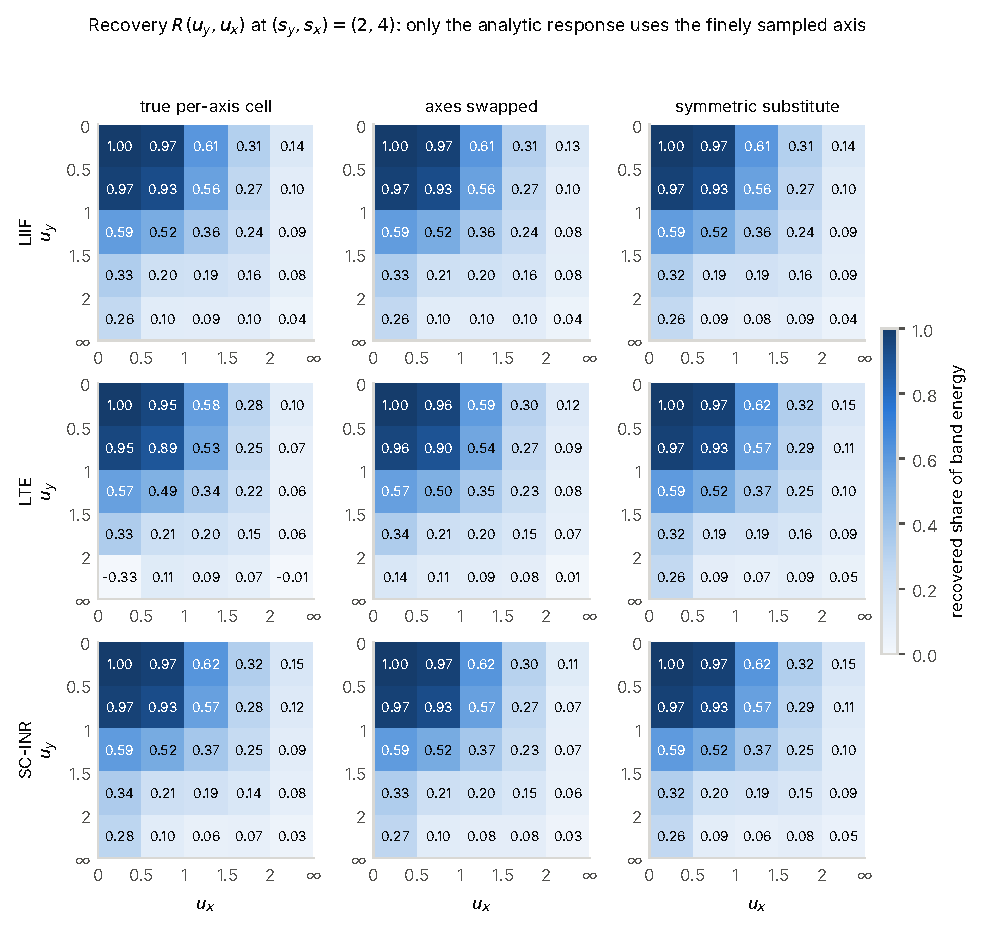
\includegraphics[width=\linewidth]{figures/fig_grid.pdf}
\caption{Recovery over $(u_y,u_x)$ for $(s_y,s_x)=(2,4)$ under the true per-axis cell, the swapped cell and the symmetric substitute (1000-epoch models, pooled over three seeds and four datasets). Only SC-INR's recovery along the finely sampled axis depends on which axis receives the fine cell; LTE's true-cell response is unidentified and even negative at high $u_y$.}
\label{fig:grid}
\end{figure}

\begin{figure}[t]\centering
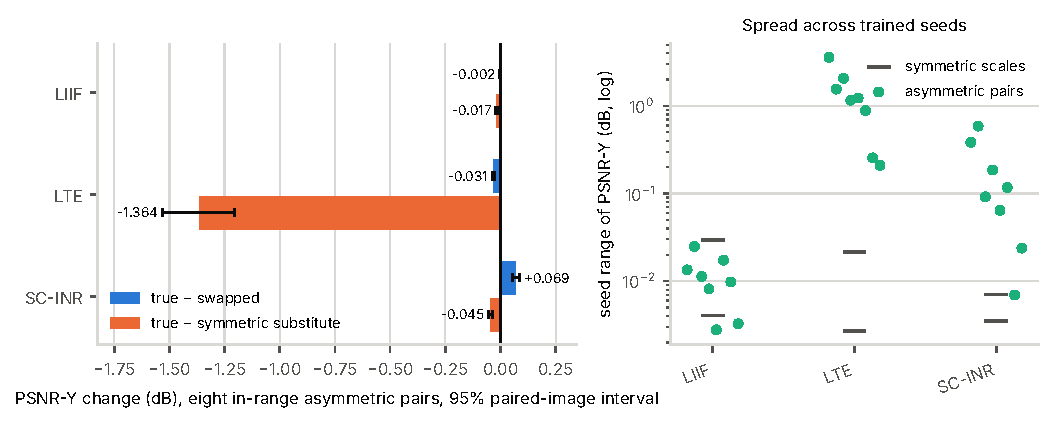
\includegraphics[width=\linewidth]{figures/fig_policy.pdf}
\caption{Left: cell-policy contrasts (Table~\ref{tab:asym}). Right: range over three seeds of the native PSNR on each asymmetric pair (dots) and at symmetric scales (bars). LTE's asymmetric response is set by the seed; SC-INR's is identified; LIIF barely uses the cell.}
\label{fig:policy}
\end{figure}

\begin{figure}[t]\centering
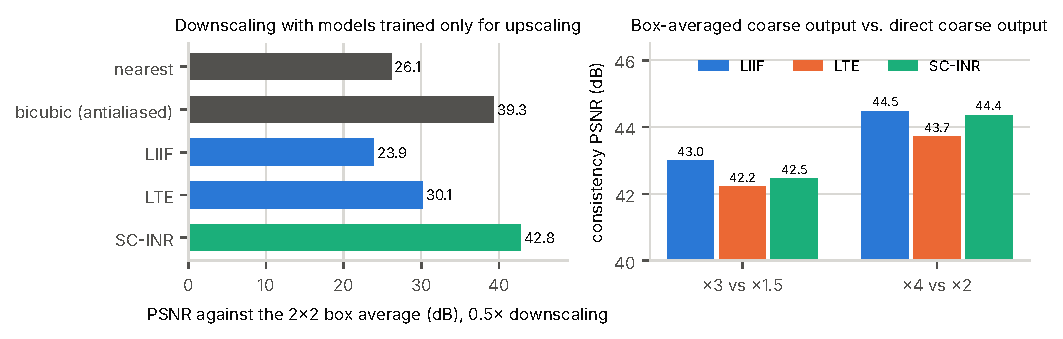
\includegraphics[width=\linewidth]{figures/fig_beyond.pdf}
\caption{Left: $0.5\times$ downscaling by models trained only for upscaling, PSNR against the box average. Right: cross-scale consistency of the three 1000-epoch decoders; the footprint-exact decoder is consistent by construction.}
\label{fig:beyond}
\end{figure}

\begin{table}[t]\centering\footnotesize
\caption{Beyond coverage. Consistency: PSNR between the $2{\times}2$ box average of the $\times4$ ($\times3$) output and the direct $\times2$ ($\times1.5$) output of the same input. Downscaling: a $240^2$ input crop queried at $0.5\times$, PSNR against the $2{\times}2$ box average and against the antialiased bicubic result. 1000-epoch models, three seeds; the footprint-exact row is by construction. \todo{add 200-epoch rows}}
\label{tab:beyond}
\begin{tabular}{lcccc}\toprule
 & \multicolumn{2}{c}{consistency (dB)} & \multicolumn{2}{c}{$0.5\times$ downscale (dB)}\\
Model & $\times4\!\to\!\times2$ & $\times3\!\to\!\times1.5$ & vs.\ box & vs.\ bicubic\\\midrule
nearest subsampling & -- & -- & 26.13 & 25.90\\
antialiased bicubic & -- & -- & 39.32 & --\\
LIIF & 44.48 & 42.99 & 23.87 & 23.81\\
LTE & 43.71 & 42.21 & 30.15 & 28.28\\
SC-INR & 44.35 & 42.46 & 42.81 & 35.47\\
Footprint-exact & $\infty$ & $\infty$ & \todo{} & \todo{}\\\bottomrule
\end{tabular}
\end{table}

\textbf{Beyond coverage (Table~\ref{tab:beyond}, Fig.~\ref{fig:beyond}).} Augmentation can cover asymmetric cells inside the training range but never footprints larger than an input pixel. Queried at $0.5\times$ with a footprint of two input pixels, SC-INR reproduces the box-averaged image at 42.8\,dB, closer than antialiased bicubic resizing itself (39.3\,dB), while LTE reaches 30.2\,dB and LIIF 23.9\,dB, below nearest-neighbour subsampling. Nothing in the training recipe, which only upscales, distinguishes the three: the difference is whether the cell is a token or an attenuation. Cross-scale consistency is violated by all three (43--44\,dB between the box-averaged fine output and the direct coarse output); the exact decoder satisfies it identically by Proposition~\ref{prop:exact}.

\textbf{Out-of-range scales.} \todo{$\times6/8/12$ table or sentence; expected convergence of all methods as the cell leverage vanishes}

\textbf{Ablations.} The no-$\sinc$ arm isolates the mechanism; LTE-linear isolates the price of the linear readout. \todo{numbers}

\begin{figure}[t]\centering
\includegraphics[width=\linewidth]{figures/fig4_qual.pdf}
\caption{Asymmetric $\times(2,4)$ and $0.5\times$ downscaling: LIIF, LTE and the footprint decoder. \todo{select by rule, e.g.\ median-gain image}}
\label{fig:qual}
\end{figure}

\section{Conclusion}
Inside the symmetric training manifold the cell is a learned token that every decoder reads equally well, and recovery profiles coincide. Outside it the token is undefined: the data never identify its per-axis response, and augmentation can only widen the manifold, not close it. Treating the cell as a footprint and integrating the representation over it analytically makes every query well defined, gives cross-scale consistency for free, and costs \todo{little} at standard scales. The analysis also sets expectations: gains from any decoder design are confined to bands near and above the input Nyquist limit.

\bibliographystyle{IEEEtran}
\bibliography{refs}
\end{document}
